\documentclass{article}

\usepackage{arxiv}

\usepackage{fontspec}
\setmainfont{Linux Libertine O}
\usepackage{bm}
\usepackage{polyglossia}
\setdefaultlanguage{english}
\setotherlanguage{russian}

\usepackage{url}
\usepackage{booktabs}
\usepackage{amsfonts}
\usepackage{amssymb}
\usepackage{amsmath}
\usepackage{nicefrac}
\usepackage{microtype}
\usepackage{lipsum}
\usepackage{graphicx}

\usepackage[numbers]{natbib}
\usepackage{amsthm}
\usepackage{doi}
\usepackage{xcolor}

\usepackage{todonotes}
\newcommand{\todoask}[1]{\todo[color=blue!40]{\textbf{Ask:} #1}}
\newcommand{\todocheck}[1]{\todo[color=green!40]{\textbf{Check:} #1}}
\newcommand{\todoread}[1]{\todo[color=orange!40]{\textbf{Read:} #1}}
\newcommand{\todocomment}[1]{\todo[color=purple!40]{\textbf{Comment:} #1}}


\title{Робастый метод детекции машинносгенерированных изображений}

% \author{%
%     Kilinkarov Georgii \\
%     Chair of Data Analysis\\
%     Moscow Institute of Physics and Technology\\
%     Moscow, Russia \\
%     \texttt{kilinkarov.gv@phystech.edu} \\
%     \And
%     Daniil Dorin  \\
%     Affiliation \\
%     Address \\
%     \texttt{email} \\
%     \AND
%     Andrey Grabovoy \\
%     Affiliation \\
%     Address \\
%     \texttt{email}
% }

\author{%
    Килинкаров Георгий \\
    Кафедра анализа данных\\
    Московский физико-технический институт(МФТИ)\\
    Москва, Россия\\
    \texttt{kilinkarov.gv@phystech.edu} \\
    \And
    Даниил Дорин  \\
    Аффиляции \\
    Адрес \\
    \texttt{email} \\
    \AND
    Андрей Грабовой \\
    Аффиляции \\
    Адрес \\
    \texttt{email}
}

\date{}

\hypersetup{
    pdftitle={Comparative Analysis of Data-Driven Approaches for Hydrological Forecasting},
    pdfsubject={cs.LG},
    pdfauthor={Eldar Khuzin, Novikov Ivan, Abramov Dmitrii},
    pdfkeywords={Flood discharge, Rainfall-runoff modeling, More}
}

\begin{document}
\maketitle

\section{Аннотация}
В связи с улучшением качества машиносгенерированных изображений становится очень сложно отличать реальное изображение от сгенерированных.  Существующие на данный момент решения имеют низкую обобщающую способность. В этой статье рассматриваются разные модели, в том числе несвязанные с нейронными сетями. Также используется вся существующая информацию и модели, для подбора наилучшего решения. Дополнительно строится модель, которая сначала проверяет метод генерации, потом уже использует конкретную модель для этого метода генерации. Помимо этого, используются методы графических редакторов, на основе искусственного интеллекта.


\keywords{Машинносгенерированные изображения}

\section{Введение}
\label{sec:introduction}

В современном мире в связи с развитием генераторов изображений человеческому глазу стало уже слишком сложно отличать настоящие изображение от машиносгенерированное. Ещё сложнее человеку отличить реальное изображение от реального, но с использованием графического редактора \cite{OnlineDetection}. В связи с доступностью этих сервисов стали очень распространены разные виды мошенничества, использующие машиногенерацию. Таким образом задача детекции машинносгенерированных изображений стала очень важна.


На данный момент не существует общего подхода к решению этой задачи, устойчивого относильно появления новых моделей. Например, появление диффузионных моделей генерации изображений свело сущесвтующие на тот момент методы к точности около 60 процентов \cite{GenImage}. Таким образом, существующие на данный момент методы имеют низкую обобщающую способность. Актуальные научные статьи на эту тему можно поделить на три типа: построение устойчивой модели с помощью добавления новых типов генерации в фазу обучения \cite{AivsAi, OnlineDetection}, решение задачи с помощью методов, не использующих AI (с помощью классических методов и рассмотрения спектра света) \cite{ZeroShot}, создание новых более мощных датасетов для данный задачи \cite{GenImage, CIFAKE}.


AI-модели обучается на всё более новых и новых датасетах, включая в себя новые способы генерации, создаются способы онлайн-обучения \cite{OnlineDetection}, что улучшает постепенно качество, но концептуально не отличается от предыдущих методов и не обеспечивает устойчивость в случае, если появится более инновационный метод генерации. До появления диффузионных моделей высокое качество показывал метод, рассматривающий спектр по Фурье \cite{ZeroShot}. Но на диффузионных моделях не показывает уже высокого качества.

Таким образом, в этой статье проводится попытка объединить существующие методы и найти новый способ детекции машиносгенерированных изображений. Новизна заключается в объединении методов и построении модели, предполагающей сначала тип генерации, а потом проверяющей на генерацию сгенерировано ли изображение уже непосредственно с предположением определенного типа генерации.

Преимущество этого подхода заключается в подборе оптимальной модели для конкретного класса генирации, проблема заключается в высокой цене ошибки: если произойдет ошибка в предсказании класса генерации, то будет использоваться заведомо плохо подходящая модель.

В качестве векторизатора мы используем предобученный CLIP \cite{CLIP}, который используется во множестве разных исследований для разных целей и задач \cite{ForClip1, ForClip2, ForClip3}, в том числе используется в качестве векторизатора для задач классификации \cite{ForClip2, ForClip3}
\section{Постановка задачи}
\label{sec:problem_statement}
Задана выборка $$\mathfrak{D} = \{\bm{x_i}, y_i \},\ i= 1, ..., N,$$ где $\bm{x_i} \in \mathbb{N}_0^{H \times W \times C}$~--- изображение размера $H \times W \times C$, $y_i \in \{ 0, 1\}.$ \\

Необходимо построить отображение $\bm{F}: \mathbb{N}_0^{H \times W \times C} \rightarrow \{ 0, 1 \}.$

Для нахождения оптимального отображения \( \bm{F}^* \) в классе моделей \( \mathcal{F} \) используется Binary Cross-Entropy Loss (BCE):
\[
	\bm{F}^* = \arg\min_{\bm{F}^* \in \mathcal{F}} \operatorname{BCE}(F).
\]

\section{Теория}
\label{sec:theory}
Отображение $\bm{F}: \mathbb{N}_0^{H \times W \times C} \rightarrow \{ 0, 1 \}.$ представляет из себя композицию двух отображений: $\bm{F} = \bm{f} \circ \bm{g}$, где:
\begin{center}
    $\bm{f}: \mathbb{N}_0^{H \times W \times C} \rightarrow \mathbb{R}^{d}$ ~--- векторизация изображения
\end{center}
\begin{center}
    $\bm{g}: \mathbb{R}^{d} \rightarrow \{ 0, 1 \}$ ~--- классификатор
\end{center}
В статье для $\bm{F}$ обучается только голова классифкатора $\bm{g}$, а $\bm{f}$ фиксировано и не обучается. Для векторизатора $\bm{f}$ рассматривается CLIP \cite{CLIP} . \\

CLIP \cite{CLIP} - модель, обученная на изображении и его текстовом представлении. На выходе получаем размер 512. Эта модель является одним из state-of-art классификаторов, для многих задач достаточно сделать голову классификатора и получится высокая точность для классификатора. \\

Одна из основный идей обучения CLIP \cite{CLIP} состоит в том, что модель при обучении использует помимо изображения ещё и её текстовое представление, которое создаётся также моделью CLIP \cite{CLIP} в другой фазе обчения. Кодировщик изображения и кодировщик текста обучаются совместно. На рисунке \ref{fig:example_one} представлен краткий процесс обучения. Для нашей задачи от  CLIP \cite{CLIP} нам нужен кодировщик изрбражения. В течение обучения использовалась серия из 5 ResNet и 3 Vision Transformer. В качестве оптимизатора используется оптимизатор Adam \cite{Adam} с регуляризатором decoupled weight decay \cite{Requl}, применяемой ко всем весам, которые являются усилителями или смещением, и затуханием скорости обучения по графику косинусов \cite{Sgd}.  \\
\begin{figure}[ht]
    \centering
    \includegraphics[width=0.8\textwidth]{CLIP_structure.png}
    \caption{Описание подхода обучения CLIP \cite{CLIP}}
    \label{fig:example_one}
\end{figure}


\section{Вычислительный эксперимент}
Целью вычислительного эксперемента является проверка качества двухступенчатой классификации. \\

В работе рассматривается датасет данных Artifact \cite{artifact}, для вычислительного эксперемента взято 13200 изображений. Датасет включается в себя реальные изображения и 25 методов генерации изображений, включая 13 GANs, 7 диффузионных, и 5 других методов генерации. Изображения по классам берутся так, чтобы их количество было одинаково для всех классов, кроме real(их очень много) и ddpm(их очень мало). Количество данных для классов на тестовой выборке можно посмотреть в таблице \ref{}


\begin{table}[h]
\centering
\footnotesize
\renewcommand{\arraystretch}{1.3}
\begin{tabular}{|l|*{13}{c|}}
\hline
Модель & \rotatebox{90}{real} & \rotatebox{90}{stylegan1} & \rotatebox{90}{stylegan2} & \rotatebox{90}{stylegan3} & \rotatebox{90}{big gan} & \rotatebox{90}{pro gan} & \rotatebox{90}{projected\_gan} & \rotatebox{90}{gau gan} & \rotatebox{90}{star gan} & \rotatebox{90}{gansformer} & \rotatebox{90}{generative inpainting} & \rotatebox{90}{mat} & \rotatebox{90}{palette} \\ \hline
Accuracy & 919 & 53 & 141 & 54 & 53 & 51 & 53 & 53 & 53 & 53 & 53 & 54 & 53  \\ \hline
\end{tabular}

\vspace{0.5cm} % Отступ между частями таблицы

% Вторая часть таблицы (13 столбцов)
\begin{tabular}{|l|*{14}{c|}}
\hline

Модель & \rotatebox{90}{tamping transformer} & \rotatebox{90}{ddpm} & \rotatebox{90}{lattent diffusion} & \rotatebox{90}{stable diffusion} & \rotatebox{90}{vq diffusion} & \rotatebox{90}{glide} & \rotatebox{90}{lama} & \rotatebox{90}{denoising diffusion gan} & \rotatebox{90}{face syntheyics} & \rotatebox{90}{clips} & \rotatebox{90}{cycle gan} & \rotatebox{90}{sfhd} & \rotatebox{90}{diffusion gan} & \rotatebox{90}{Общее}\\ \hline
Accuracy & 54 & 6 & 53 & 53 & 53 & 53 & 54 & 53 & 53 & 53 & 53 & 53 & 53 & 2287 \\ \hline
\end{tabular}
\caption{Таблица количества данных для разных классов генерации на тестовой выборке. На тренировочном тоже самое, только данных больше.}\label{tab:my_table}
\end{table}


В качестве основной модели будет использоваться CLIP \cite{CLIP}.
Выборка была поделена на обучающую и тестовую в соотношении 70 на 30. \\

В работе рассматривается несколько разных моделей для сравнения и на основе этих эксперементов выбирается лучшая. За базовую модель была взята модель с CLIP \cite{CLIP} бинарным классификатором. Вторая модель к CLIP \cite{CLIP} добавляет два линейных слоя с функцией активацией Relu Один линейный слой с выходом 26(именно столько классов изображений существует в датасете). Третья модель является многоклассовым классификатором, но Test Accuracy считается для возможности сравнения как для бинарной модели. На Рисунке \ref{fig:models_scheme} представлена схема разных моделей.\\

\begin{figure}[ht]
    \centering
    \includegraphics[width=0.8\textwidth]{3_models_sheme.png}
    \caption{Общая схема для трех разных основных эксперементов: слева базовый, посередине модель с дополнительным слоем, а справа многоклассовая классификация. Значком снежинки обозначено то, что мы не обучаем CLIP \cite{CLIP}, используем то, что уже существует.}
    \label{fig:models_scheme}
\end{figure}




Для оценки качества модели используются следующие оценочные метрики: Accuracy, Recall, Precision, ROC-AUC, PR-curve. Эти метрики помогают в проверке качества моделей и сравнения моделей между собой. Для многоклассовой классификацией также рассматривается confusion matrix для понимаю природы ошибок и слабых мест модели. Модели сравниваются по всем выше перечисленным метрикам, а также по графику обучения, включающие в себя 3 графика: график Loss от номера эпохи, Train, Test Accuracy от номера эпохи и время, затраченное на backward и forward от номера эпохи.\\

Обучение происходит с помощью оптимизатора Adam \cite{Adam}, с критерием CrossEntropy и 20 эпохами. 



\subsection{Базовая модель}
Была обучена базовая модель по описанному выше общему принципу на 20 эпохах. Результаты Accuracy разных классов представлены в Таблице \ref{tab:my_table}.\\

Для более полного понимания были построены Roc-Auc и PR-curve. Это представлено на Рисунке \ref{fig:base_roc}.\\


\begin{table}[h]
\centering
\footnotesize
\renewcommand{\arraystretch}{1.3}
\begin{tabular}{|l|*{13}{c|}}
\hline
Модель & \rotatebox{90}{real} & \rotatebox{90}{stylegan1} & \rotatebox{90}{stylegan2} & \rotatebox{90}{stylegan3} & \rotatebox{90}{big gan} & \rotatebox{90}{pro gan} & \rotatebox{90}{projected\_gan} & \rotatebox{90}{gau gan} & \rotatebox{90}{star gan} & \rotatebox{90}{gansformer} & \rotatebox{90}{generative inpainting} & \rotatebox{90}{mat} & \rotatebox{90}{palette} \\ \hline
Accuracy & 0.48 & 0.64 & 0.75 & 0.50 & 1.00 & 0.78 & 0.96 & 1.00 & 0.94 & 0.92 & 0.75 & 0.74 & 0.66 \\ \hline
\end{tabular}

\vspace{0.5cm} % Отступ между частями таблицы

% Вторая часть таблицы (13 столбцов)
\begin{tabular}{|l|*{14}{c|}}
\hline

Модель & \rotatebox{90}{tamping transformer} & \rotatebox{90}{ddpm} & \rotatebox{90}{lattent diffusion} & \rotatebox{90}{stable diffusion} & \rotatebox{90}{vq diffusion} & \rotatebox{90}{glide} & \rotatebox{90}{lama} & \rotatebox{90}{denoising diffusion gan} & \rotatebox{90}{face syntheyics} & \rotatebox{90}{clips} & \rotatebox{90}{cycle gan} & \rotatebox{90}{sfhd} & \rotatebox{90}{diffusion gan} & \rotatebox{90}{Общее}\\ \hline
Accuracy & 0.703 & 1.00 & 0.91 & 0.62 & 0.92 & 0.88 & 0.87 & 0.54 & 1.00 & 1.00 & 0.98 & 0.98 & 0.84 & 0.69 \\ \hline
\end{tabular}
\caption{Таблица accuracy для разных классов. Верным классом для класса генерации здесь мы считаем, если модель предсказала, что это изображение является машинносгенерированным.}\label{tab:my_table}
\end{table}



\begin{figure}[ht]
    \centering
    \includegraphics[width=0.8\textwidth]{base_Roc_Pr.png}
    \caption{Roc-Auc и PR-curve для базовой модели}
    \label{fig:base_roc}
\end{figure}

Помимо всего прочего был проведен анализ изображений, на которых наша базовая модель ошибается для учета этих ошибок и доработок. Рисунок \ref{fig:fake_image} демонстрирует эти ошибки. \\

\begin{figure}[ht]
    \centering
    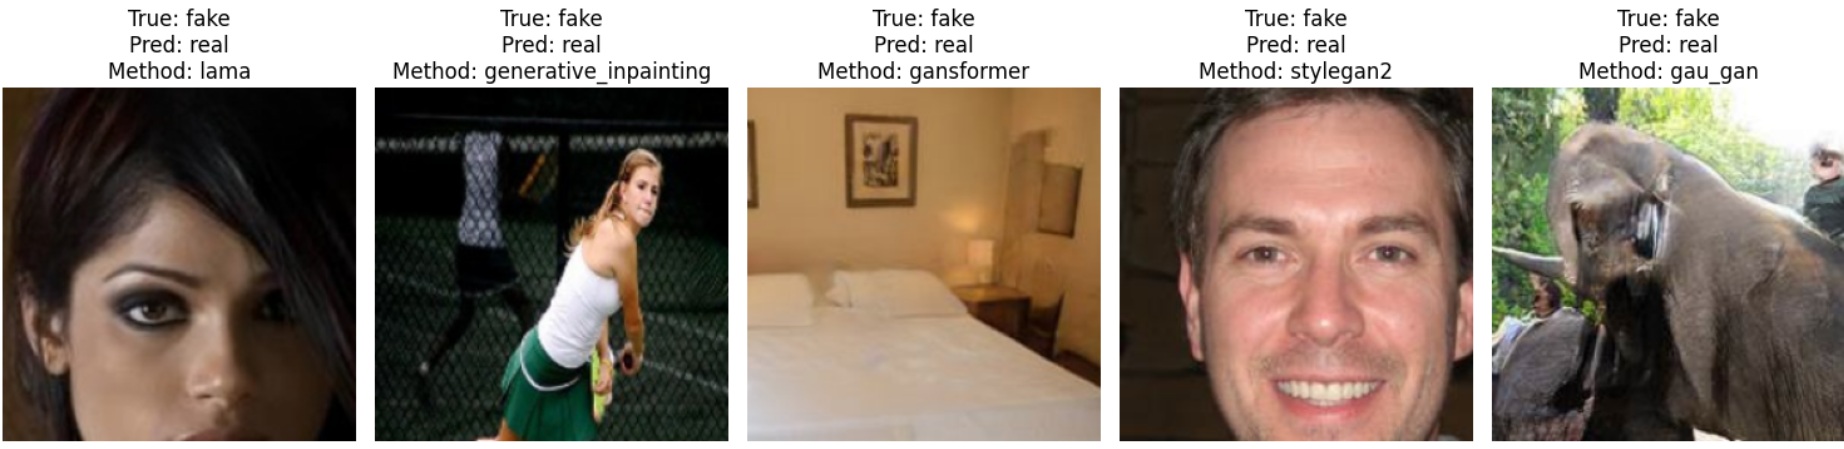
\includegraphics[width=0.8\textwidth]{fake_images.png}
    \caption{Примеры ошибок базовой модели}
    \label{fig:fake_image}
\end{figure}


\subsection{Модель с дополнительным слоем}
Также было проведено сравнение первых двух моделей. Сравниваем по 3 графикам: график Loss от номера эпохи, график Accuracy от номера эпохи и время на проходы от номера эпохи. \\
Рисунок \ref{fig:2_models_train} показывает насколько добавление слоя улучшело модель при таком же времени работы.

\begin{figure}[ht]
    \centering
    \includegraphics[width=0.8\textwidth]{train_curve.png}
    \caption{Сравнение первых двух моделей}
    \label{fig:2_models_train}
\end{figure}


\subsection{Модель многоклассовой классификации}
Модель многоклассовой классификации обучается на 5 эпохах с критерием - CrossEntropy с весами. В анализе считается, что модель предсказала правильно в случае, если реальное предсказано моделью как реальное, а сгенерированное как сгенерированное без учета конкретных классов генерации. Таки образом мы получаем сопостовимые для анализа модели. На Рисунке \ref{fig:3_models_train} представлено сравнение моделей. Как видим результат неудовлитворительный, так как модель многоклассовой классификации практически не обучилась. Для анализа проблем была рассмотрена confusion matrix (Рисунок \ref{fig:confusion}).

\begin{figure}[ht]
    \centering
    \includegraphics[width=0.3\textwidth]{3_models_train.png}
    \caption{Сравнение первых трех моделей}
    \label{fig:3_models_train}
\end{figure}

\begin{figure}[ht]
    \centering
    \includegraphics[width=0.8\textwidth]{confusion_matrix.png}
    \caption{Confusion matrix для модели многоклассовой классификации.}
    \label{fig:confusion}
\end{figure}

\bibliographystyle{unsrtnat}
\bibliography{references}
\end{document}
